% Mai Ha Vu
% Linguistics paper template
% uses dvi-ps-pdf-chain to compile

\documentclass[english, 11pt]{article}

%\usepackage{etex}
\usepackage[T1]{fontenc}
\usepackage{charter}
\usepackage[utf8]{inputenc}
\usepackage[usenames,dvipsnames,svgnames,table]{xcolor}
\usepackage{babel}
\usepackage[bottom = 1in, left=1in, right=1in]{geometry}
\usepackage{fancyhdr}	%for headers and footers
\pagestyle{fancy}
\usepackage{natbib}  %use if there are citations!
\usepackage{tipa}   %for IPA
\usepackage{amstext} 
\usepackage{amsmath}
\usepackage{qtree}    %for trees
\usepackage{tikz}
\usepackage{tikz-qtree}
\usepackage{stmaryrd} 
\usepackage{arydshln} 
\usepackage[colorlinks=true]{hyperref}
\usepackage{OTtablx}	%for OT tableaux. See below for example.
\usepackage{pifont} %for symbols
\usepackage{dsfont}	%for more symbols
\usepackage{gb4e} 	%for linguistic examples and glosses

\newcommand{\vs}{\vspace{11pt}}		%makes a vertical skip of 12pts
\newcommand{\underscore}{\underline{\hspace{0.5cm}}}		%0.5 cm long underline
%\let\eachwordtwo=\sc

\begin{document}

\rfoot{\thepage}	%page number in right foot
\cfoot{}
\rhead{Mai Ha Vu}	%right header
\lhead{Linguistics}	%left header


\title{Linguistics paper}	%title of the document
\author{Mai Ha Vu}		%author of the document
%\date{November 3, 2013}		%date. comment out if you want current date.


\maketitle		%prints the title

\section{This is a section} %to get rid of numbering, use \section*

\section*{This is a section without numbers}

\subsection{And you can have subsections too!}

\subsubsection{And subsubsections}

	
	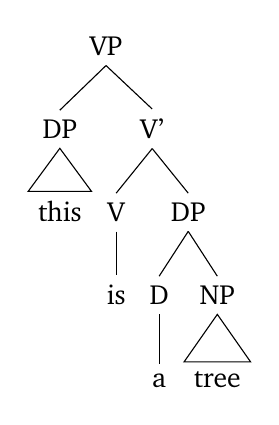
\begin{tikzpicture}
	
	\Tree [.VP  [.DP \edge[roof];this ] [.V' [.V is ] [.DP [.D a ] [.NP \edge[roof];tree ] ] ]]
	\end{tikzpicture}
	
	
	
	
	\vs 
	
\section{Here is some gloss (from my own Syntax homework)}


\begin{exe}
	\ex 
	\begin{xlist}
		\ex[]{
		\gll B{\o}rnene har set denne film. \\
			Children-the have seen this film. \\}\label{first}
		\ex[]{
		\gll Denne film har b{\o}rnene set. \\
			This film have children-the seen. \\}\label{second}
		\ex[*]{
		\gll Denne film b{\o}rnene har set. \\
			This film children-the have seen. \\}\label{third}
		\ex[*]{
		\gll Har b{\o}rnene set denne film. \\
			Have children-the seen this film. \\}\label{fourth}
	\end{xlist}
\end{exe}

And you can even refer to your example sentences, like this: \ref{first}, \ref{second}, \ref{third}, and \ref{fourth}.



\section{Want to do phonetic transcription?}

\textipa{l2tEk k\ae n h\ae nd@l T\ae P t\super hu}! 


\section{Tables}

\begin{tabular}{l | c | c} \hline \hline
here & is & a \\ \hline 
cute & table& ! \\ \hline \hline
\end{tabular}

\section{Citations}

Here's an example of a citation \citep{lol}.

Or here: \cite{lol}.

\bibliographystyle{chicago}
\bibliography{template}
\end{document} 